\documentclass[12pt]{article}

\usepackage[utf8]{inputenc}
\usepackage{latexsym,amsfonts,amssymb,amsthm,amsmath}
\usepackage{tikz}
\usepackage{stanli}
\usetikzlibrary{shapes,calc,through,3d,patterns}
\usetikzlibrary{arrows.meta,decorations.pathreplacing,angles,quotes}
\usepackage{multicol}
\usepackage{geometry}
\usepackage{mathtools}
\usepackage{siunitx}
\usepackage{booktabs}

\setlength{\parindent}{0in}
\setlength{\oddsidemargin}{-0.25in}
\setlength{\textwidth}{7in}
\setlength{\textheight}{9.3in}
\setlength{\topmargin}{-1in}
\setlength{\headheight}{18pt}

\newcommand\blfootnote[1]{%
    \begingroup
    \renewcommand\thefootnote{}\footnote{#1}%
    \addtocounter{footnote}{-1}%
    \endgroup
}

\definecolor{darkred}{rgb}{0.6,0,0}

\newcommand{\bolddelta}{\boldsymbol\delta}
\newcommand{\boldxi}{\boldsymbol\xi}

\begin{document}

\noindent ME473 - Dynamic finite element analysis of structures\hfill EPFL\\
Stefano Burzio \hfill 2025\\
\vspace{0.3cm}

\hspace*{\fill}\textbf{\Large Problem set 2 - solutions}\hspace*{\fill}

\hrulefill

\subsection*{Problem 1}
\textbf{Weak form:} The integral form for the longitudinal vibrations of a free bar is
$$\int_0^{\ell} E A\left(\frac{\partial^2 u_1}{\partial x^2}\right) \delta u_1\, dx=\int_0^{\ell} \rho A \ddot{u}_1 \delta u_1\, dx$$
where $\delta u_1$ represents a virtual displacement along the axis $Ox$ and it does not depends on time. Integration by parts of the left-hand side of the previous equation leads to the expression:
\begin{equation*}
    -\int_0^{\ell} E A\left(\frac{\partial u_1}{\partial x}\right)\left(\frac{\partial \delta u_1}{\partial x}\right)\, dx+\left[E A\left(\frac{\partial u_1}{\partial x}\right) \delta u_1\right]_0 ^{\ell}=
    \int_0^{\ell} \rho A \ddot{u}_1 \delta u_1\, dx
\end{equation*}

Since the boundary terms vanish at $x=0$ and $x=\ell$ due to the homogenous boundary conditions: $EA \, \partial_{x} u_1(0, t)=EA \, \partial_{x} u_1(\ell, t) = 0$, the weak form of the problem reduces to finding the longitudinal displacement $u_1(\cdot,t) \in H^1(]0, \ell[)$ for every $t \in[0, T]$, such that the following equations are satisfied for every $\delta u_1 \in H^1(]0, \ell[)$
        \begin{equation}
            \label{wf}
            \int_0^{\ell} E A\left(\frac{\partial u_1}{\partial x}\right)\left(\frac{\partial \delta u_1}{\partial x}\right)\, dx+
            \int_0^{\ell} \rho A \ddot{u}_1 \delta u_1\, dx=0
        \end{equation}
        with the initial conditions expressed in integral form:
        \begin{equation}
            \label{ic}
            \begin{aligned}
                 & \int_0^{\ell} \rho A u_1\left(x, 0\right) \delta u_1\, dx=
                \int_0^{\ell} \rho A u_{0} \delta u_1 \, d x                          \\
                 & \int_0^{\ell} \rho A \dot{u}_1\left(x, 0\right) \delta u_1 \, d x=
                \int_0^{\ell} \rho A {v}_{0} \delta u_1 \, d x
            \end{aligned}
        \end{equation}
        Note that both the real and virtual displacements do not vanish at both the ends of the bar.
        \vspace{0.3cm}

        \textbf{Two-terms Galerkin approximation:} The Galerkin approximation of the problem entails determining an approximation \( u_1^h(\cdot,t) \in H^1 \subset H^1(]0, \ell[) \) for all \( t \in [0, T] \), such that equations \eqref{wf} and \eqref{ic} hold with \( u_1 \) replaced by \( u_1^h \) and $\mathcal U=\mathcal V=H^1(]0, \ell[)$ replaced by $\mathcal U^{h}=\mathcal V^{h}$. Here $\mathcal U^{h}$ denotes a finite-dimensional subspace of $\mathcal U$.

We assume for the approximated real and virtual axial displacements the two-terms expansions:
\begin{equation}\label{approx}
    \begin{aligned}
        u_1^h(x,t)        & =h_1(x) q_1(t)+h_2(x) q_2(t)=\mathbf{H} \mathbf{q}(t)                     \\
        \delta u_1^h(x,t) & =h_1(x)  \delta q_1 +h_2(x)  \delta q_2 =\mathbf{H} \bolddelta \mathbf{q}
    \end{aligned}
\end{equation}
in which $\mathbf{H}=\left[h_1, h_2\right]$ is the row matrix $(1 \times 2)$ of shape functions, generating a basis of $\mathcal U^{h}$. Moreover, $\mathbf{q}(t)=\left\{q_1(t), q_2(t)\right\}^{\mathrm{T}}$ along with the associated $\bolddelta \mathbf{q}=\left\{\delta q_1, \delta q_2\right\}^{\mathrm{T}}$ denote the vectors of discrete longitudinal displacements, real and virtual respectively, along the axis $Ox$.

By inserting the approximations \eqref{approx} into equation \eqref{wf}, we obtain:
\begin{equation*}
    \bolddelta \mathbf{q}^{\mathrm{T}}\left\{\left[\int_0^{\ell} E A\left(\frac{\partial \mathbf{H}^{\mathrm{T}}}{\partial x}\right)\left(\frac{\partial \mathbf{H}}{\partial x}\right) \mathrm{d} x\right] \mathbf{q}(t)+
    \left[\int_0^{\ell} \rho A \mathbf{H}^{\mathrm{T}} \mathbf{H} \, d x\right] \ddot{\mathbf{q}}(t)\right\}=0
\end{equation*}
Since this expression must hold for any $\bolddelta \mathbf{q}$, the semi-discrete weak form consists of solving the following matrix equation for $\mathbf{q}(t), t \in[0, T]$, along with initial conditions:
\begin{equation*}
    \begin{aligned}
         & \mathbf{M} \ddot{\mathbf{q}}(t)+\mathbf{K} \mathbf{q}(t)=\mathbf{0}                           \\
         & \mathbf{q}(0)=\mathbf{M}^{-1} \int_0^{\ell} \rho A \mathbf{H}^{\mathrm{T}} u_{0} \, d x       \\
         & \dot{\mathbf{q}}(0)=\mathbf{M}^{-1} \int_0^{\ell} \rho A \mathbf{H}^{\mathrm{T}} v_{0} \, d x
    \end{aligned}
\end{equation*}
where the components of the $(2 \times 2)$ mass matrix $\mathbf{M}$ and stiffness matrix $\mathbf{K}$ are given by:
\begin{equation*}
    \begin{aligned}
         & m_{i j}=\int_0^{\ell} \rho A h_i(x) h_j(x) \, d x \quad (i, j=1,2)              \\
         & k_{i j}=\int_0^{\ell} E A h_{i}^\prime(x)h_{j}^\prime(x)\,  dx \quad (i, j=1,2)
    \end{aligned}
\end{equation*}
As mentionned in the statement of the problem, let us select the following polynomial shape functions:
$$
    \begin{aligned}
         & h_1(x)=1        \\
         & h_2(x)=x / \ell
    \end{aligned}
$$
By introducing these expressions into the coefficients $m_{i j}$ and $k_{i j}$, and after integrating the terms, the semi-discrete weak form can be rewritten as the following linear system of differential equations of 2nd order:
\begin{equation}\label{sdwf}
    \frac{\rho A \ell}{6}\left[\begin{array}{ll}
            6 & 3 \\
            3 & 2
        \end{array}\right] \ddot{\mathbf{q}}(t)+\frac{E A}{\ell}\left[\begin{array}{ll}
            0 & 0 \\
            0 & 1
        \end{array}\right] \mathbf{q}(t)=\mathbf{0}
\end{equation}
It is well known in the theory of discrete vibratory systems that the solution to be sought for the discrete displacement vector is of the harmonic type:
$$
    \mathbf{q}(t)=\mathbf{p} \alpha \cos (\omega t-\varphi)
$$
where $\alpha$, $\omega$, and $\varphi$ represent, respectively, the reference amplitude, the angular frequency, and the phase of the sinusoidal function, and where $\mathbf{p}=\left\{p_1, p_2\right\}^{\mathrm{T}}$ is a vector with constant coefficients.

Based on this harmonic form, the system of differential equations \eqref{sdwf} is replaced by the homogeneous algebraic system of two equations with two unknowns $\omega$ and $\mathbf p$:
$$
    \left(\frac{\omega^2 \rho A \ell}{6}\left[\begin{array}{ll}
            6 & 3 \\
            3 & 2
        \end{array}\right]-\frac{E A}{\ell}\left[\begin{array}{ll}
            0 & 0 \\
            0 & 1
        \end{array}\right]\right) \mathbf{p}=\mathbf{0}
$$

The characteristic equation
$$
    \omega^2\left(\omega^2 \ell^2 / 12-E / \rho\right)=0
$$
admits the following two solutions, corresponding to the two approximate natural frequencies of the structure:
$$
    \begin{aligned}
         & \omega_1=0                                                                           \\
         & \omega_2=\sqrt{12} \sqrt{\frac{E}{ \rho \ell^2}}=3.464 \sqrt{\frac{E}{ \rho \ell^2}}
    \end{aligned}
$$
The first natural frequency, corresponds to a rigid body axial mode and is therefore zero. The second natural frequency relates to the fundamental traction-compression mode of the bar and deviates by approximately $10 \%$ from the exact value, which is given by $\omega_2^{\text{exact}} =\pi \sqrt{E / \rho \ell^2}$.

It is important to note that the natural frequencies of a system are intrinsic properties determined by its mass and stiffness distribution. They do not depend on the initial conditions, which only affect the amplitude and phase of the system's response but not the frequencies themselves.

\subsection*{Problem 2}
We begin by deriving the weak form and subsequently discretizing it. Following the standard procedure, we multiply the differential equation in its strong form by a virtual axial displacement, \(\delta u_1\), integrate over the spatial domain, and apply integration by parts. This yields the following expression:
\begin{equation*}
    -\int_0^{\ell} E A\left(\frac{\partial u_1}{\partial x}\right)\left(\frac{\partial \delta u_1}{\partial x}\right)\, dx+\left[E A\left(\frac{\partial u_1}{\partial x}\right) \delta u_1\right]_0 ^{\ell}=\int_0^{\ell} \rho A \ddot{u}_1 \delta u_1\, dx
\end{equation*}
By enforcing the homogeneous boundary condition at \( x = 0 \) and the inhomogeneous boundary condition at \( x = \ell \), the boundary term can be simplified, resulting in the following expression:
\begin{equation*}
    \label{wfpb2}
    \int_0^{\ell} E A\left(\frac{\partial u_1}{\partial x}\right)\left(\frac{\partial \delta u_1}{\partial x}\right)\, dx+ku_{1}(\ell,t)\delta u_{1}+
    \int_0^{\ell} \rho A \ddot{u}_1 \delta u_1\, dx=0
\end{equation*}
Discretizing the equation using the Galerkin procedure leads to the following mass and stiffness matrices:
\begin{equation*}
    \begin{aligned}
         & m_{i j}=\int_0^{\ell} \rho A h_i(x) h_j(x) \, d x \quad (i, j=1,2)                                        \\
         & k_{i j}=\int_0^{\ell} E A h_{i}^\prime(x)h_{j}^\prime(x)\,  dx +k h_{i}(\ell)h_{j}(\ell) \quad (i, j=1,2)
    \end{aligned}
\end{equation*}

The code below, which can be found on the \texttt{MATLAB} drive of the course, computes the stiffness and mass matrices for the system using two different set of shape functions, and then solves the generalized eigenvalue problem to determine the natural frequencies.

The parameters are defined below:
\begin{verbatim}
clc; clear; close all;
% Define symbolic variables
syms x
% l: length of bar
l = 2                  
% E: modulus of elasticity
E = 210e9              
% rho: density
rho = 7850             
% k: spring characteristic constant 
k = 12e3                
% A: area of cross section
beta=4/15                
A = 150e-6 * (1 - beta * x/l) 
\end{verbatim}

We defines symbolic variables for shape functions (\texttt{H\_poly}, \texttt{B\_poly}, \texttt{H\_harmonic}, \texttt{B\_harmonic}) used to compute the stiffness and mass matrices. It is important to note that when selecting the harmonic shape functions, we must ensure that \( u_1^h \) vanishes at \( x = 0 \). Consequently, this imposes the condition \( h_i(0) = 0 \), which leads us, for the harmonic approximation, to selecting only sinusoidal functions. As for the frequency of the sinusoidal function, there are no imposed constraints. However, since the displacement is not zero at \( x = \ell \), it is advisable to choose frequencies that do not cause the sinusoidal function to vanish at this location. A common choice to slightly simplify the computations is to select only frequencies that ensure the function \( h_i \) attains a unitary value at \( x = \ell \):
$$h_{i}(x)=\sin\Big(\frac{(2i-1)\pi}{2\ell}x\Big)\quad (i=1,2)$$
Let us visalize the shape functions.
\begin{verbatim}
fplot(H_poly,[0,l]);
grid
xlabel('x');
legend('Polynomial shape functions', Location='southeast');
axis padded;

fplot(H_harm,[0,l]);
grid
xlabel('x');
legend('Harmonic shape functions', Location='southeast');
axis padded;
\end{verbatim}
\begin{figure}[h!]
    \centering
    \begin{minipage}{0.45\textwidth}
        \centering
        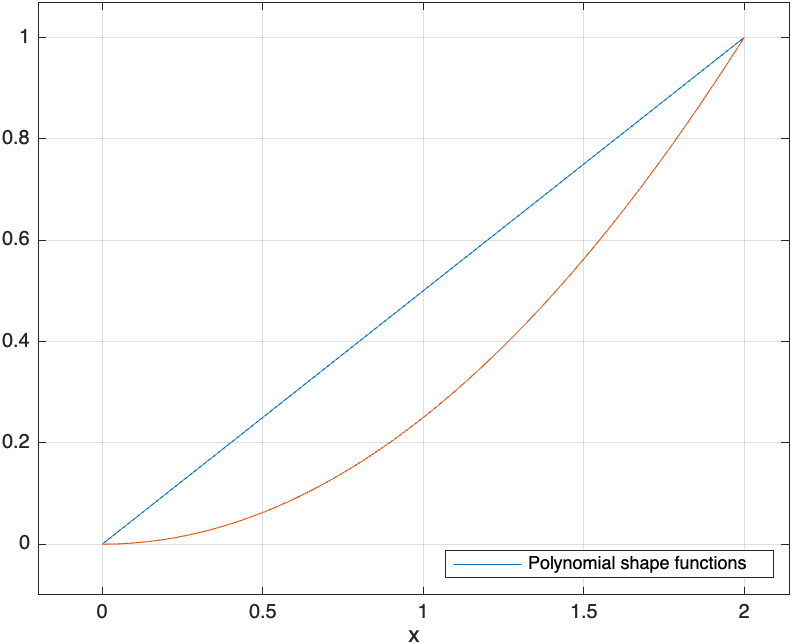
\includegraphics[width=\linewidth]{../images/polyShape.png}
    \end{minipage}
    \hfill
    \begin{minipage}{0.45\textwidth}
        \centering
        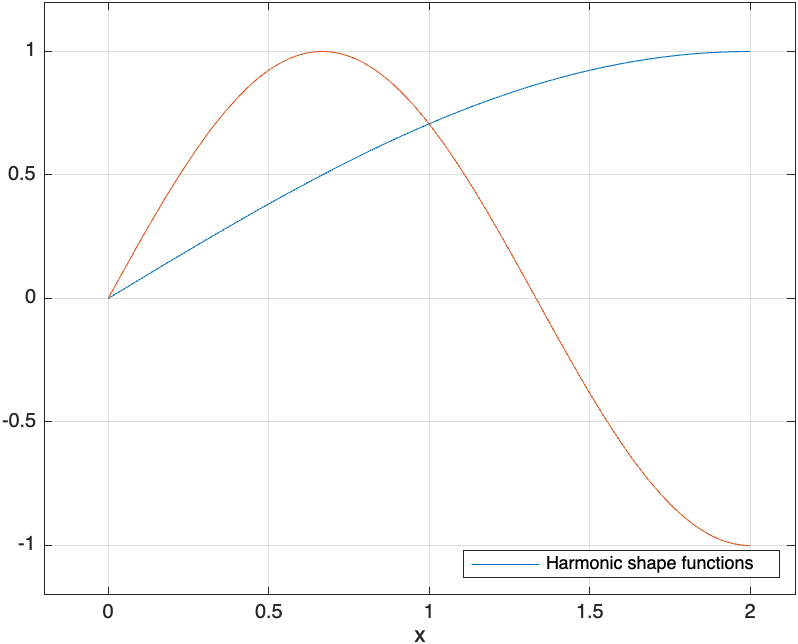
\includegraphics[width=\linewidth]{../images/harmShape.png}
    \end{minipage}
\end{figure}

The loop below defines two sets of shape functions: polynomial and harmonic.
\begin{verbatim}
syms H_poly B_poly H_harm B_harm                     
for i=1:2                  
    H_poly(:,i)=(x/l).^i;
    B_poly(:,i)=x.^(i-1).*i/l^i;

    H_harm(:,i)=sin(pi/(2*l)*(2*i-1)*x);
    B_harm(:,i)=pi/(2*l)*(2*i-1)*cos(pi/(2*l)*(2*i-1)*x);
end 
\end{verbatim}
The stiffness matrix is calculated using the shape functions and material properties. The integrals over the length of the bar are computed as:
\begin{verbatim}
K_poly=int(E*A*transpose(B_poly)*B_poly,x,[0 l]) 
	   + k*transpose(subs(H_poly,x,l))*subs(H_poly,x,l);
K_harm=int(E*A*transpose(B_harm)*B_harm,x,[0 l]) 
	  + k*transpose(subs(H_harm,x,l))*subs(H_harm,x,l);
\end{verbatim}
Similarly, the mass matrix is calculated using the shape functions and the density of the material:
\begin{verbatim}
M_poly=int(rho*A*transpose(H_poly)*H_poly,x,[0 l]);    
M_harm=int(rho*A*transpose(H_harm)*H_harm,x,[0 l]);    
\end{verbatim}
The generalized eigenvalue problem is solved for both the polynomial and harmonic cases to obtain the natural frequencies:
\begin{verbatim}
eigenvalues_poly = eig(double(K_poly),double(M_poly));
eigenvalues_harm = eig(double(K_harm),double(M_harm));
\end{verbatim}

The \texttt{eig} function computes the eigenvalues of the generalized eigenvalue problem, which represent the square of the natural frequencies. The eigenvalues are extracted and used the square root is taken to obtain the natural frequencies:

\begin{verbatim}
omega_poly_approx = sqrt(eigenvalues_poly)  
omega_harm_approx = sqrt(eigenvalues_harm)
\end{verbatim}




\end{document}